% !TeX root = main.tex
\section*{Results and discussion}
The mask was made with a variety of shapes in different sizes including -- but not limited to -- checkerboards, outward radiating lines and shapes with optical proximity correction (OPC). The complete design is shown in figure \ref{fig:litho_design} In this section only the checkerboard shapes are discussed as the other shapes did not contribute to more insight. A more complete overview of microscope images of the designed shapes can be found in appendix \ref{ap:inspec_img}.

To find the optimal exposure time $\tau$, the checkerboard pattern of each sample is inspected under an optical microscope. With a positive tone resist, under exposure results in not enough resist being dissolved in the development solution (figure \ref{fig:b3d1}). Of the exposed areas, the molecules near the boundary do not reach the dose threshold, while the molecules in the center do. This is because the molecules in the center receive much scattered light from neighbouring molecules, molecules near the boundary do not nearly have as many neighbours. When the resist is exposed for too long, boundary areas underneath the opaque parts of the mask also go above the dose threshold (figure \ref{fig:b3a1}). With the limited amount of developed samples, an exposure time of 2 minutes was found to be optimal (figure \ref{fig:b3e1}). 

% ================== Checked up to here ===============
Several images of the positive tone sample with an exposure time of 2 minutes were taken with a Hitachi S4800 scanning electron microscope. These are shown in figures \ref{fig:b2d5_q5}-\subref{fig:b2d10_q11}:

\begin{figure*}[!t]
    \centering
    \begin{subfigure}[t]{0.24\linewidth}
    	\centering
    	\resizebox{\linewidth}{!}{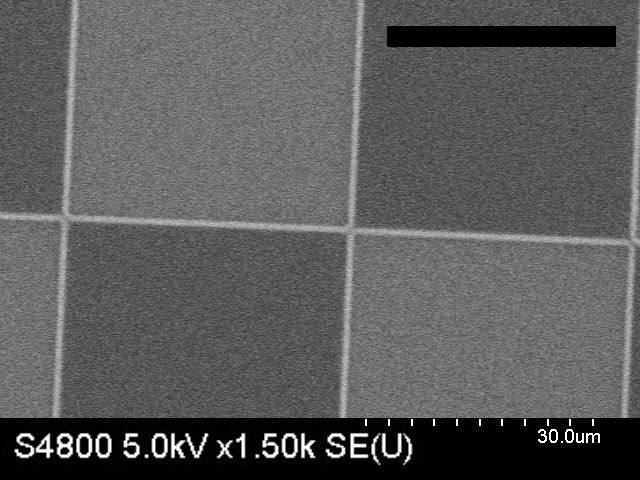
\includegraphics{data/sem/b3a5_q05.jpg}}
    	\caption{Structure size of $\sim$35. Black scale bar is 30.0~$\mu$m wide.}
    	\label{fig:b2d5_q5}
    \end{subfigure}
    \hfill
    \begin{subfigure}[t]{0.24\linewidth}
    	\centering
    	\resizebox{\linewidth}{!}{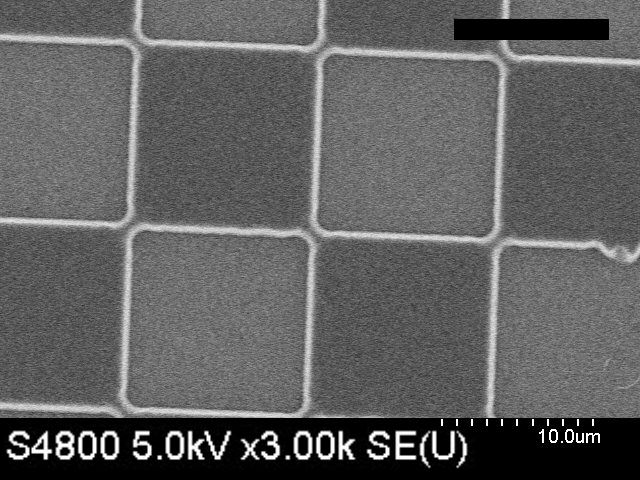
\includegraphics{data/sem/b3a7_q07.jpg}}
    	\caption{Structure size of $\sim$10 $\mu$m. Slight overexposure can be seen at the vertices of the squares. Black scale bar is 10.0~$\mu$m wide.}
    	\label{fig:b2d7_q7}
    \end{subfigure}
    \hfill
    \begin{subfigure}[t]{0.24\linewidth}
    	\centering
    	\resizebox{\linewidth}{!}{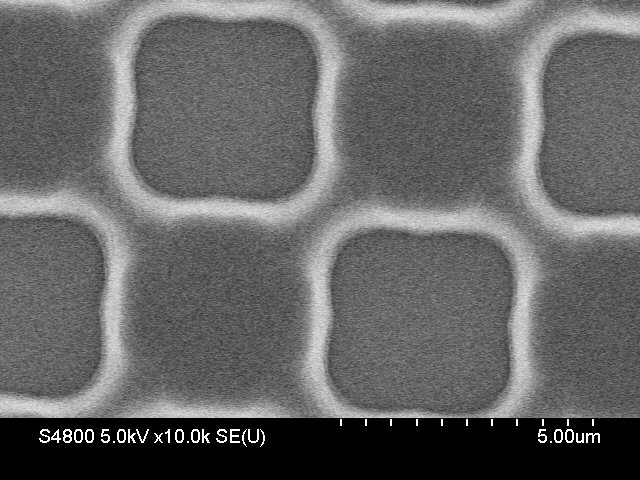
\includegraphics{data/sem/b3a9_q09.jpg}}
    	\caption{Structure size of $\sim$4 $\mu$m. The effects of overexposure become pronounced at structure sizes of $\sim$4 $\mu$m. Black scale bar is 5.00~$\mu$m wide.}
    	\label{fig:b2d9_q9}
    \end{subfigure}
    \hfill
    \begin{subfigure}[t]{0.24\linewidth}
    	\centering
    	\resizebox{\linewidth}{!}{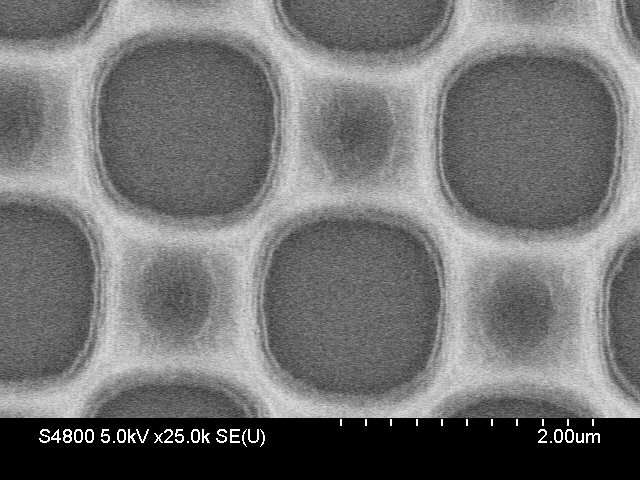
\includegraphics{data/sem/b3a10_q11.jpg}}
    	\caption{For structure sizes $\sim$1 $\mu$m the patterns lose recognizability. Black scale bar is 2.00~$\mu$m wide.}
    	\label{fig:b2d10_q11}
    \end{subfigure}
    \caption{SEM images of the positive tone sample with an exposure time of 2 minutes}
\end{figure*}
\begin{figure*}[!b]
    \centering
    \begin{subfigure}[t]{0.3\linewidth}
        \centering
        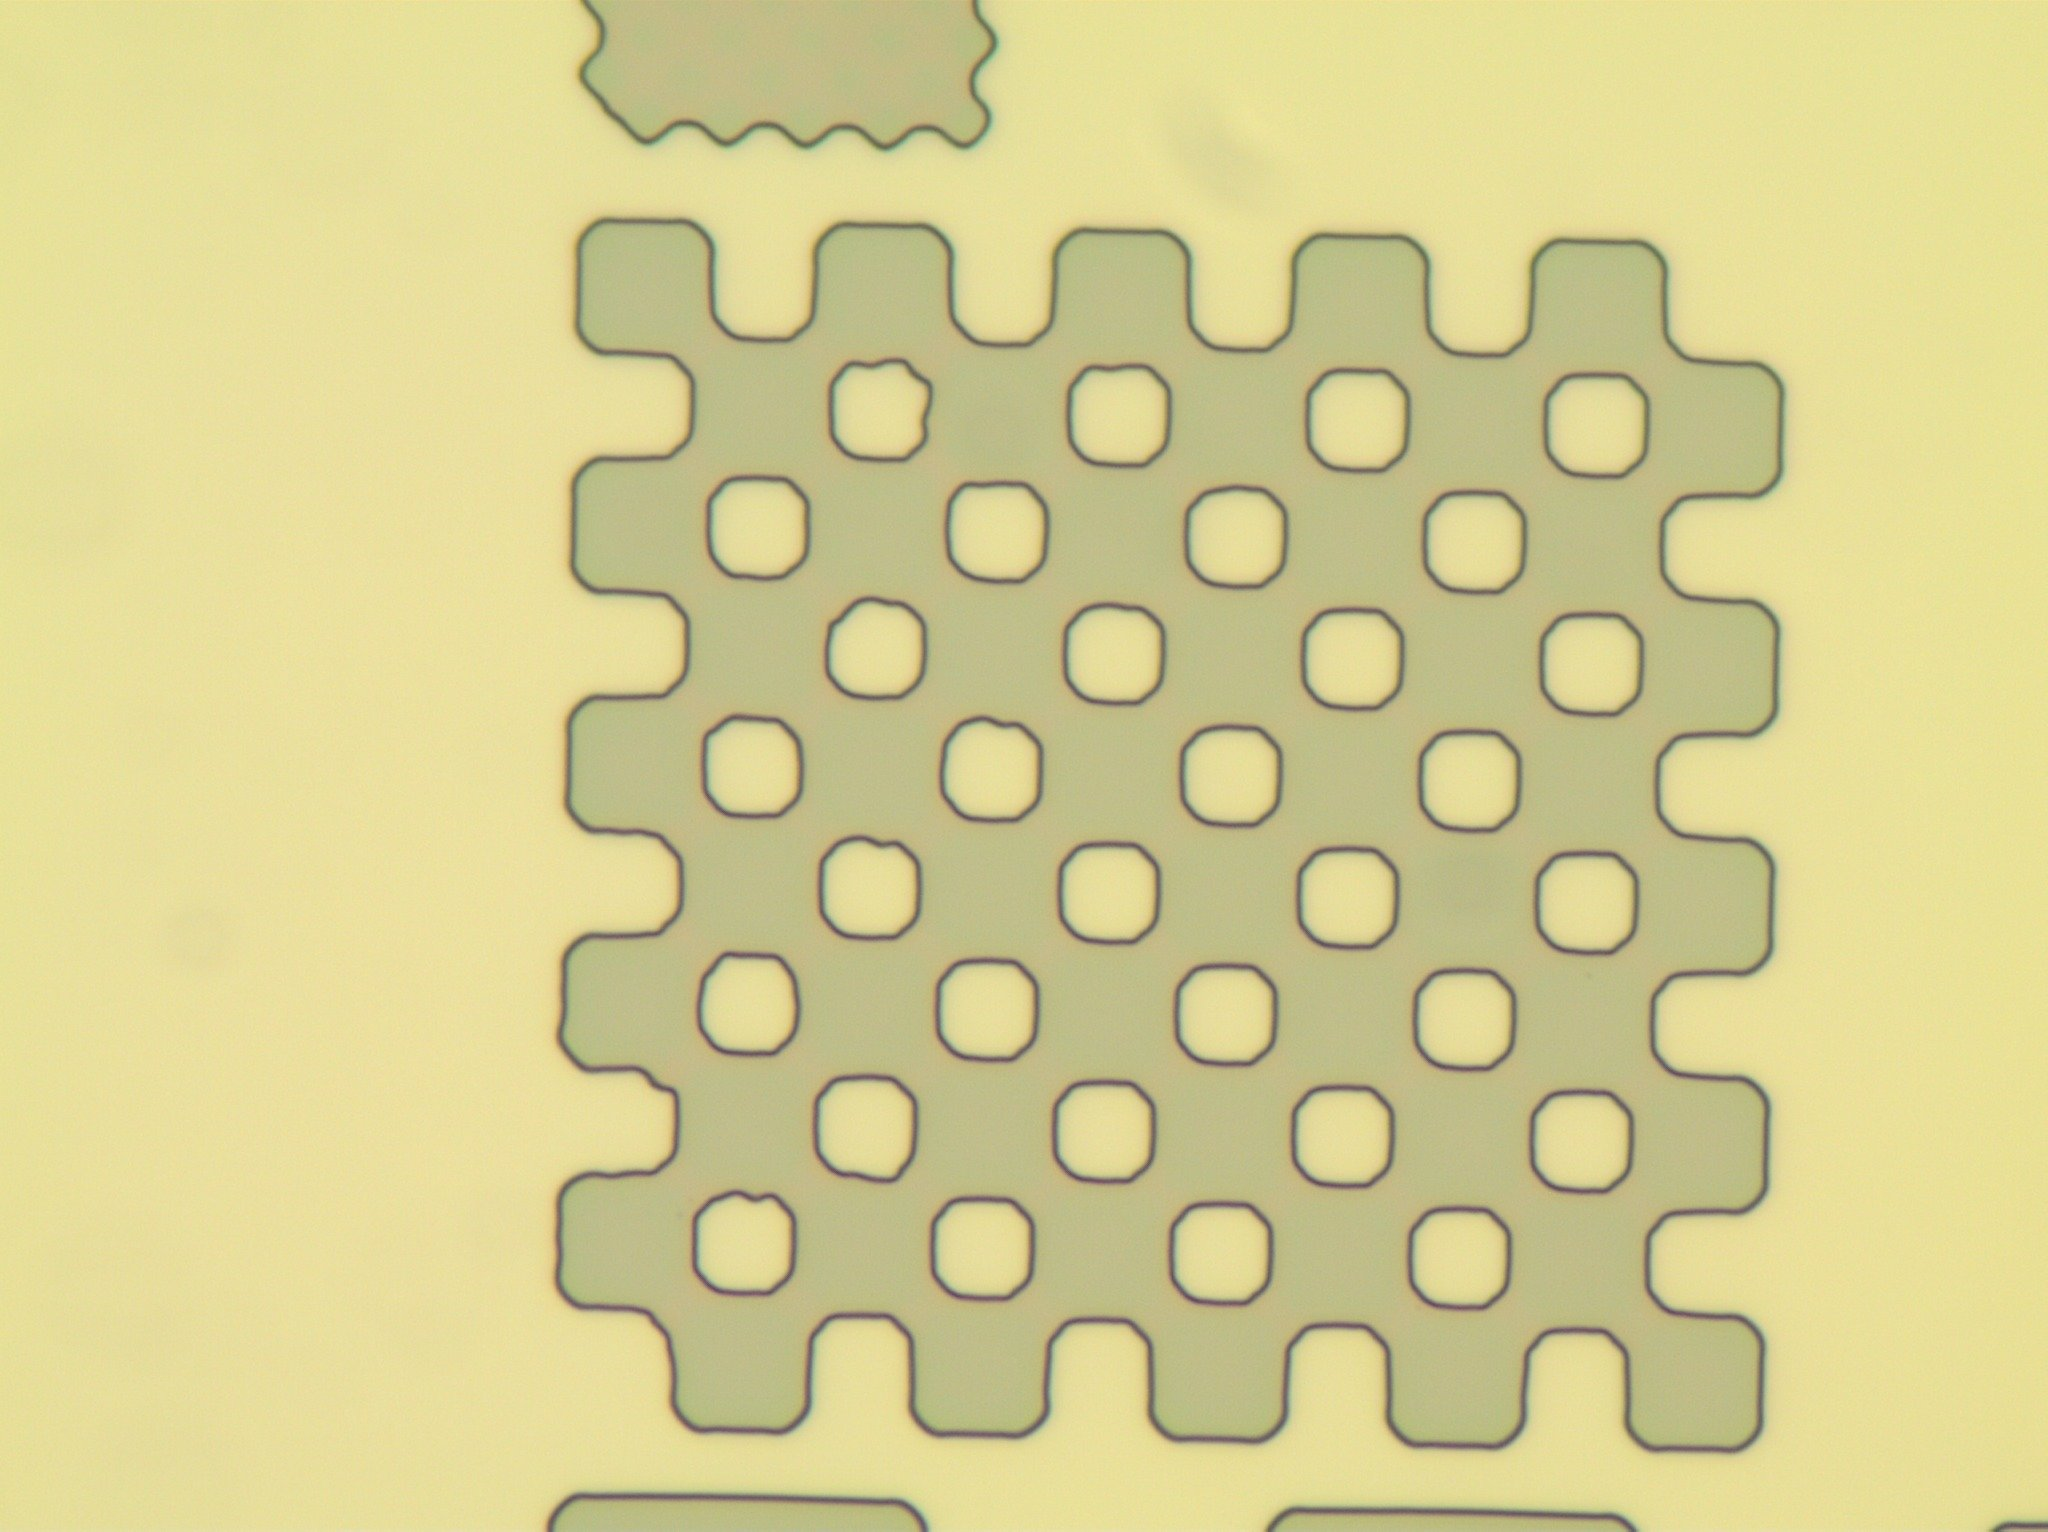
\includegraphics[width=\textwidth]{data/b2d1.jpg}
	    \caption{Sample of the negative resist pattern with an exposure time of 0.5 minutes.Taking into account that a negative tone was used, it can be seen that the sample was clearly overexposed.}
	    \label{fig:b2d1}
    \end{subfigure}
    \hfill
    \begin{subfigure}[t]{0.3\linewidth}
        \centering
        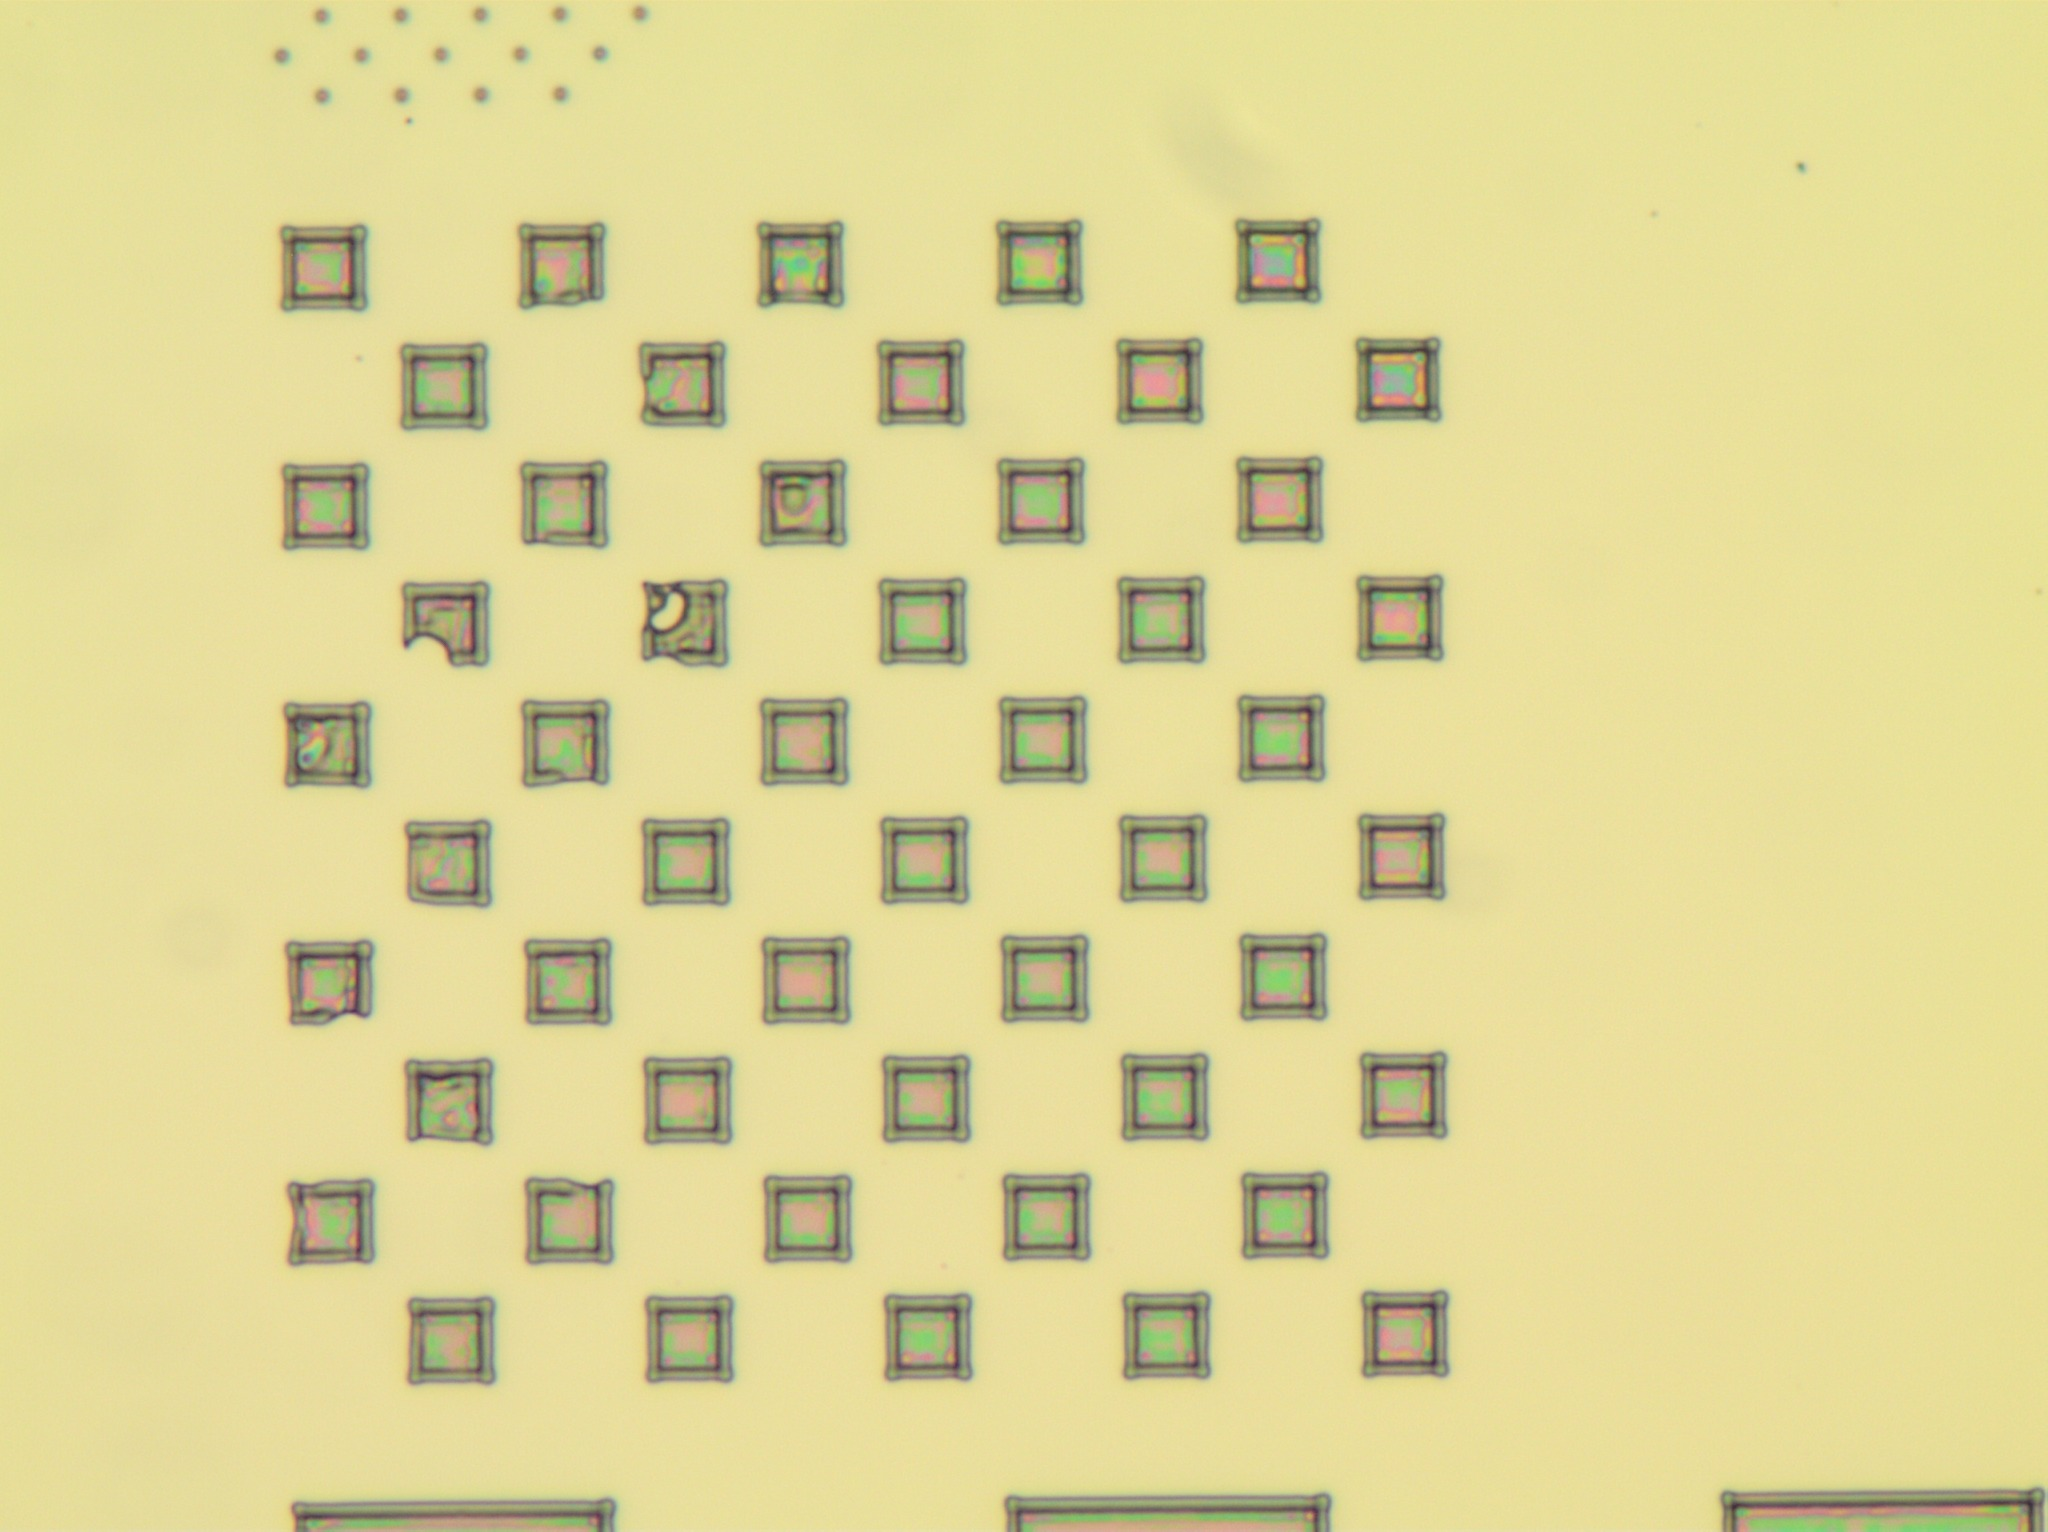
\includegraphics[width=\textwidth]{data/b2h1.jpg}
	    \caption{Sample of the negative resist pattern with an exposure time of 0.2 minutes. Note that the sample is underexposed.}
	    \label{fig:b2h1}
    \end{subfigure}
    \hfill
    \begin{subfigure}[t]{0.3\linewidth}
        \centering
        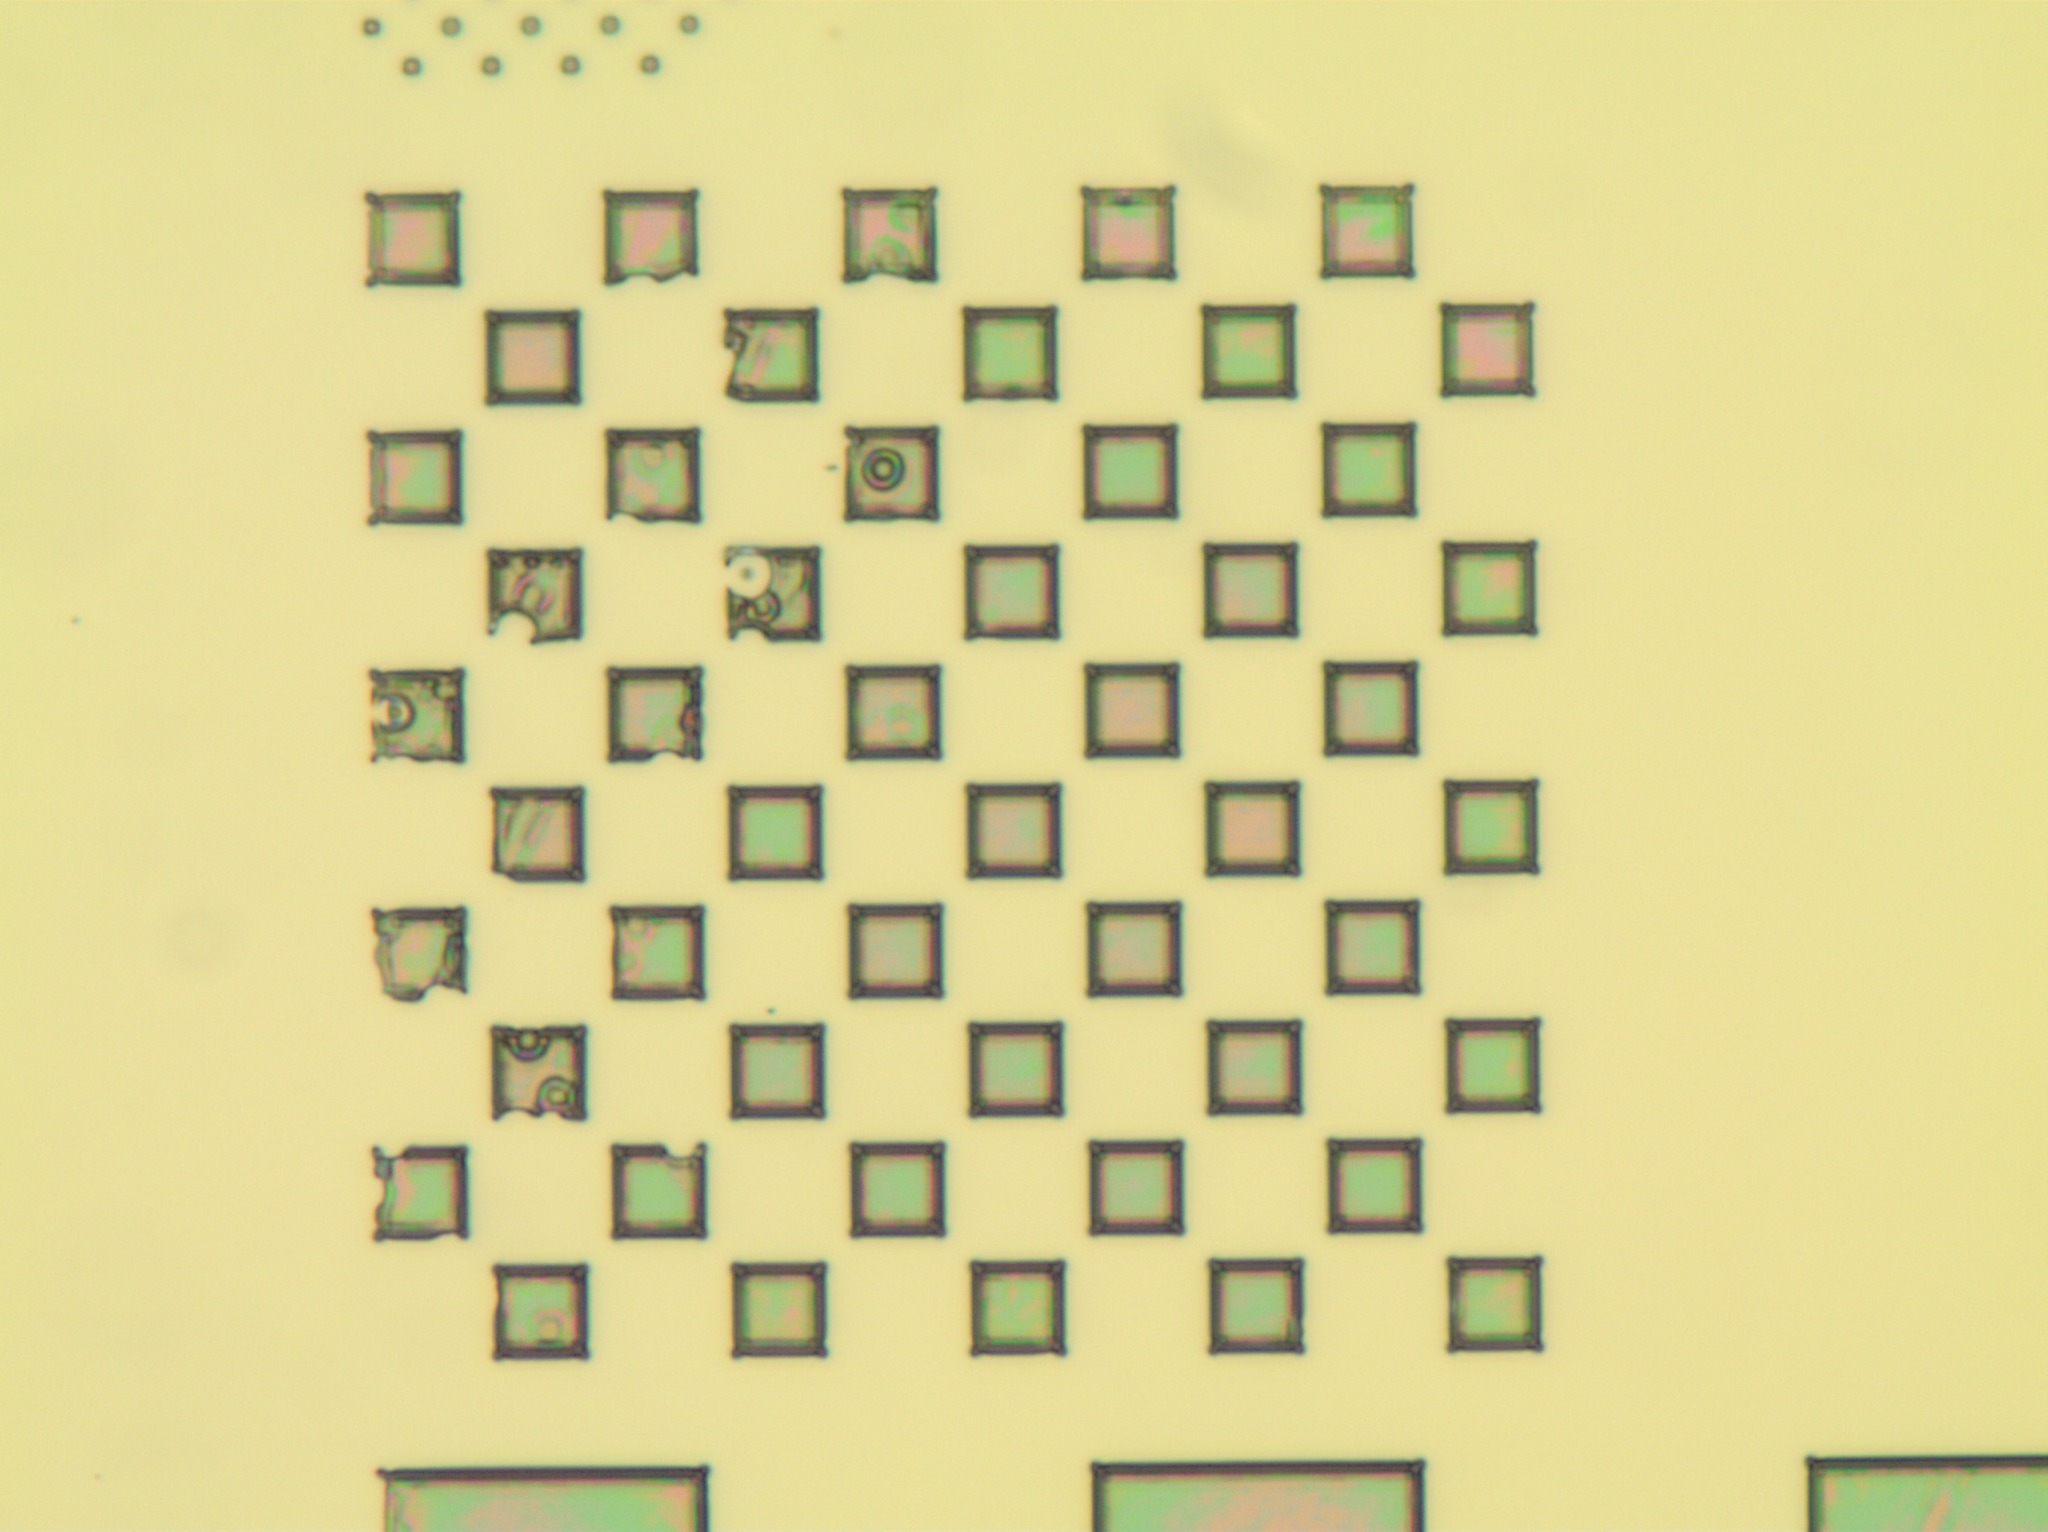
\includegraphics[width=\textwidth]{data/b2i1.jpg}
	    \caption{Sample of the negative resist pattern with an exposure time of 0.3 minutes. The sample is again underexposed, but not as much as the sample with an exposure time of 0.2 minutes.}
	    \label{fig:b2i1}
    \end{subfigure}
    \caption{Negative tone resist with different exposure times.}
\end{figure*}

The checkerboard pattern starts to decline in resolution between lengths of 2 and 10 $\mu$m. The images taken with the SEM show the same decline in resolution between 2 and 10 $\mu$m, as can be seen in the appendix.


It was found that for the negative recipe an exposure time of 0.1 minute resulted in no pattern creation at all, while exposure times of 0.5 minutes and longer resulted in overexposure of the pattern. The results of the developed samples with exposure times between 0.1 and 0.5 minutes are shown in figures \ref{fig:b2d1}, \ref{fig:b2h1} and \ref{fig:b2i1}:


From this we conclude that when using image reversal with the AZ~5214E an exposure time of around 0.4 minutes will be optimal for lithography. Images of the checkerboard pattern of the sample with an exposure time of 0.5 minutes under the Hitachi S4800 SEM are seen below:


\begin{figure*}[htb]
    \begin{subfigure}[t]{0.24\linewidth}
    	\centering
    	\resizebox{\linewidth}{!}{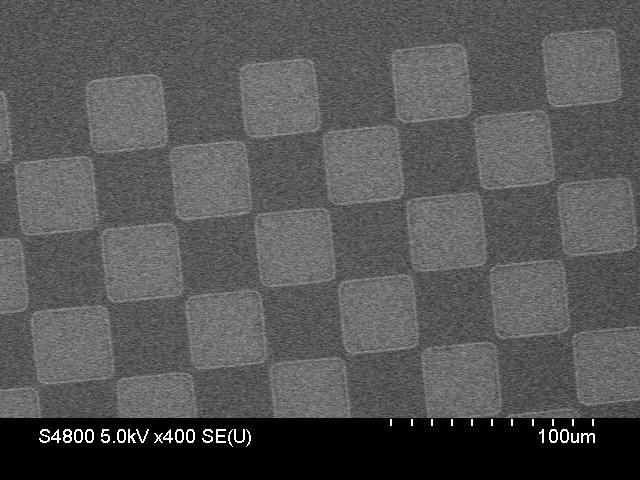
\includegraphics{data/sem/b2d26_q26.jpg}}
    	\caption{SEM. Scale bar is 100~$\mu$m}
    	\label{fig:b2d26_q26}
    \end{subfigure}
    \hfill
    \begin{subfigure}[t]{0.24\linewidth}
    	\centering
    	\resizebox{\linewidth}{!}{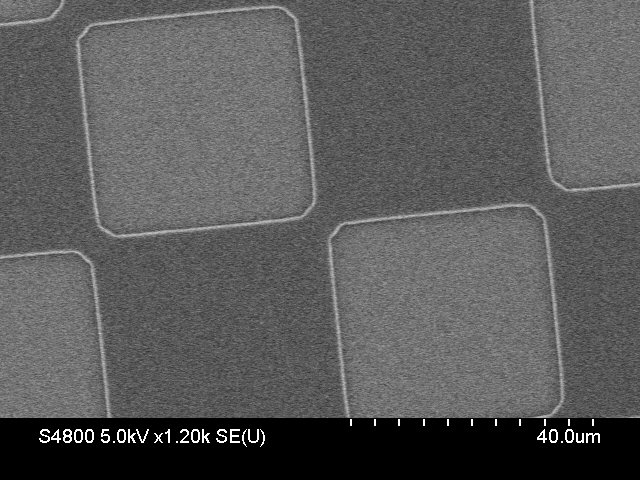
\includegraphics{data/sem/b2d27_q27.jpg}}
    	\caption{SEM. Scale bar is 40~$\mu$m}
    	\label{fig:b2d27_q27}
    \end{subfigure}
    \hfill
    \begin{subfigure}[t]{0.24\linewidth}
    	\centering
    	\resizebox{\linewidth}{!}{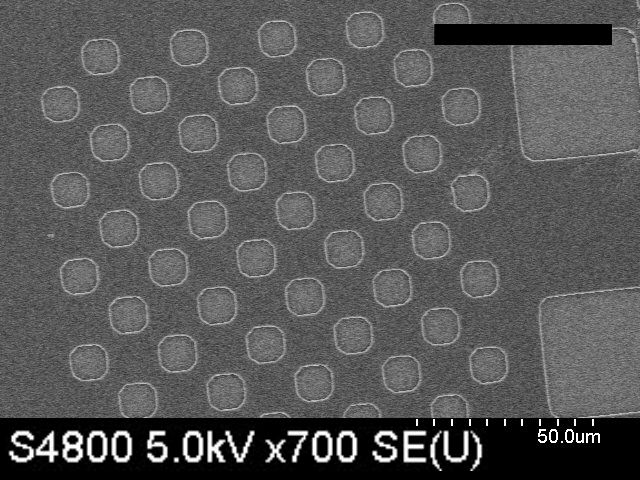
\includegraphics{data/sem/b2d28_q28.jpg}}
    	\caption{SEM. Scale bar is 50~$\mu$m}
    	\label{fig:b2d28_q28}
    \end{subfigure}
    \hfill
    \begin{subfigure}[t]{0.24\linewidth}
    	\centering
    	\resizebox{\linewidth}{!}{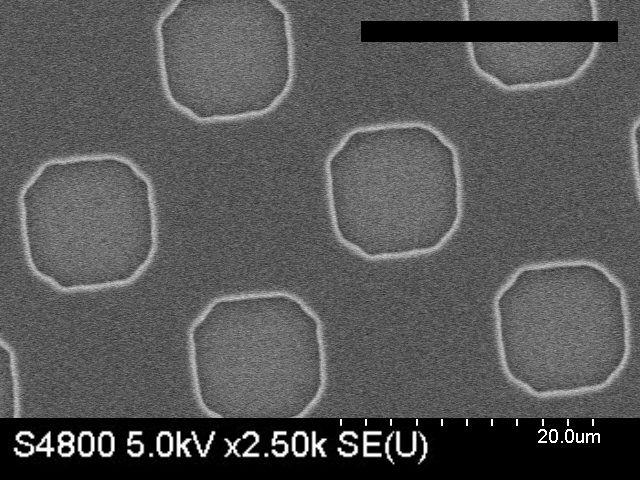
\includegraphics{data/sem/b2d29_q29.jpg}}
    	\caption{SEM. Scale bar is 20~$\mu$m}
    	\label{fig:b2d29_q29}
    \end{subfigure}
\end{figure*}


The samples were also analyzed under a profilometer.

\begin{table}[H]
    \centering
    \caption{Positive tone resist thickness}
    \begin{tabular}{X l l l}
        $\tau$ (min)& $\Delta h$ ($\mu$m) \\ 
        \hline\hline
        3.0 & 1.5932(2) \\
        4.0 & 1.6696(3) \\
        1.0 & 0.3175(3) \\
        2.5 & 1.6286(4) \\
        3.5 & 1.5920(3) \\
        \hline
    \end{tabular}
    \label{tab:pos_profile}
\end{table}

\begin{table}[H]
    \centering
    \caption{Negative tone resist thickness}
    \begin{tabular}{X l l l l}
	$\tau_1$ (min) & $\tau_2$ (min) & $\Delta h$ ($\mu$m) \\ 
        \hline\hline
        0.5 & 3.0 & 1.3845(2) \\
        1.0 & 3.0 & 1.4822(2) \\
        1.5 & 3.0 & 1.6816(2)  \\
        0.5 & 4.0 & 1.5371(2)  \\
        1.0 & 4.0 & 1.5552(3)  \\
        1.5 & 4.0 & 1.5381(2)  \\
        % 0.1 & 4.0 & 45.047  &   ~       \\
        0.2 & 4.0 & 0.8637(2)  \\
        0.3 & 4.0 & 0.5664(2)  \\
        \hline
    \end{tabular}
    \label{tab:neg_profile}
\end{table}

It is clear from the table that the positive sample with an exposure time of  1 minute and the negative sample with an exposure time of 0.1 minutes almost had no activation of the photosensitive resist. No significant overcut was detected under the profilometer for the positive samples. The possible undercut was not measured for the negative samples.
While the exposure time is of importance, the development time also plays a role. During the analyzing of a batch of positive resist samples, it was found that the quality of the samples fluctuated, and that in general longer exposure times were required. 


\todo[inline]{Images of the checkerboard pattern for all samples can be found in the appendix.}

\todo[inline]{Other parts of the recipe could also have needed adjustment as a result of a different exposure time. Further more some samples turned out to be of inferior quality because they were recycled. This combined with the limited time available, resulted in not finding a a good recipe for both the positive and negative tone resist.}

Quisque ut semper orci. Suspendisse egestas nunc augue, in pharetra enim varius eget. Vestibulum vitae placerat urna, ac vulputate ipsum. Quisque ullamcorper lectus est, eu viverra lectus vestibulum et. Suspendisse pulvinar magna urna, vitae iaculis enim sagittis id. Mauris ultricies libero sed ipsum varius vehicula. Sed dignissim mi quis ultricies feugiat. Maecenas mattis ultricies dictum. In sed interdum risus.

Quisque ut semper orci. Suspendisse egestas nunc augue, in pharetra enim varius eget. Vestibulum vitae placerat urna, ac vulputate ipsum. Quisque ullamcorper lectus est, eu viverra lectus vestibulum et. Suspendisse pulvinar magna urna, vitae iaculis enim sagittis id. Mauris ultricies libero sed ipsum varius vehicula. Sed dignissim mi quis ultricies feugiat. Maecenas mattis ultricies dictum. In sed interdum risus.